%% ── Section 4: Experimental Setup ───────────────────────────
\section{Experimental Setup}
\label{sec:experiments}

\subsection{Dataset and Preprocessing}

All methods are evaluated on the \textbf{DDR dataset}~\cite{li2019ddr}, which
contains 13,673 fundus photographs, of which 12,522 are gradable. After removing
the ungradable images, 6,260 training, 2,503 validation and 3,759 test images
remain. All images are resized to $224 \times 224$ pixels. During local training,
random horizontal flips, rotations of up to $\pm 15^{\circ}$, and mild colour
jitter are applied to reduce overfitting. The training set is strongly imbalanced:
Grade~0 (50.0\%), Grade~1 (5.0\%), Grade~2 (35.8\%), Grade~3 (1.9\%), and Grade~4
(7.3\%). For external validation, the APTOS 2019 dataset~\cite{aptos2019} is used:
3,662 labelled fundus photographs collected in India and graded on the same 0--4
scale. A public copy resized to $224 \times 224$ pixels is used, and these images
are never used for training or model selection.

\subsection{Modeling Clinical Heterogeneity}

The data are split across $K = 5$ clients in three ways, shown in
Fig.~\ref{fig:distributions}. In the figure, each bar is one client. Its segments
show the share of each DR grade among that client's images, from light (Grade~0)
to dark (Grade~4), and the number under each client label is the client's total
number of images.
\begin{itemize}[leftmargin=*,noitemsep,topsep=2pt]
  \item \textbf{IID partition:} images are assigned uniformly at random (1,252 per
  client). This is the easiest case for FL.
  \item \textbf{Dirichlet non-IID ($\alpha=0.1$):} the skew is generated with a
  Dirichlet distribution $p_k \sim \mathrm{Dir}(\alpha)$. With $\alpha=0.1$, most
  clients draw their images almost entirely from a single grade. Client sizes
  range from 32 to 2,087 images: Client~0 holds only 32 images (100\% Grade~0),
  and Client~4 holds 2,087 images, 98\% of them Grade~2.
  \item \textbf{Real-site clinical partition:} images are assigned using fixed
  grade profiles that model five types of clinic: Site~0 (general screening
  clinic; 40\% of images, 84\% Grade~0), Site~1 (rural primary care; 22\%, mainly
  Grades~0 and~2, with the largest Grade~1 share at 11\%), Site~2 (specialist
  referral eye hospital; 10\%, the largest Grade~3--4 share at 38\%), Site~3
  (diabetic retinopathy clinic; 19\%, 67\% Grade~2), and Site~4 (urban hospital;
  9\%, mixed grades).
\end{itemize}

%% FULL-WIDTH FIGURE: Per-client grade distributions
%% (placed after its description — Reviewer #3, comments 3 and 6)
\begin{figure*}[t]
  \centering
  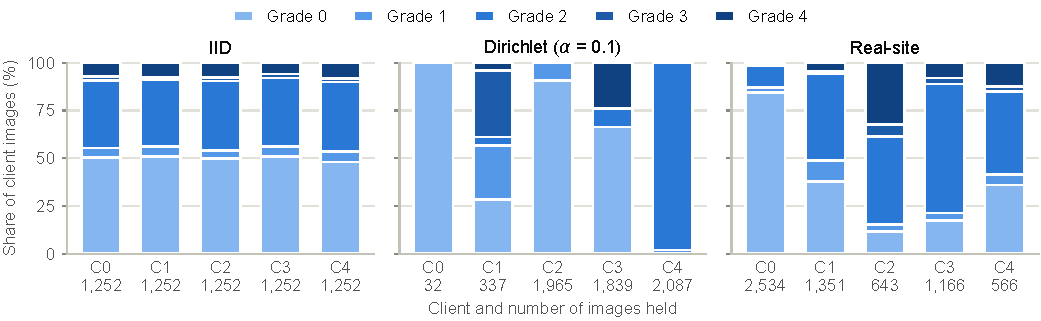
\includegraphics[width=\textwidth]{fig5_distributions.pdf}
  \caption{\normalsize Grade mix of each client under the IID, Dirichlet
  ($\alpha=0.1$) and real-site partitions. Under $\alpha=0.1$, client sizes range
  from 32 images (Client~0, 100\% Grade~0) to 2,087 images (Client~4, 98\% Grade~2).
  The real-site partition models five types of clinic, from screening clinics to
  specialist referral centres.}
  \label{fig:distributions}
\end{figure*}

\subsection{Network Architecture and Baselines}

All federated experiments use an EfficientNet-B3 backbone, which offers a good
balance between model size and accuracy at $224 \times 224$ resolution. As in a real
deployment that adapts pre-trained weights, all FL runs start from a centralised
model trained for 30 epochs (best validation QWK = 0.834, reached at epoch~23).
OrdinalFed is compared with:
(1)~a \textbf{Centralised Baseline}; (2)~\textbf{FedAvg}~\cite{mcmahan2017fedavg};
(3)~\textbf{FedProx}~\cite{li2020fedprox} with proximal coefficient $\mu = 0.01$;
and (4)~\textbf{AccWt}, an accuracy-weighted baseline based on server-side
validation scoring~\cite{bejenar2023aggregation}. AccWt uses the same schedule and
softmax weighting as OrdinalFed (Eqs.~\ref{eq:beta}--\ref{eq:weights}), but it
scores each client by plain accuracy on $\mathcal{V}$ instead of QWK, and its
clients train with class-weighted cross-entropy. A fifth configuration,
\textbf{OrdinalFed + Prox}, adds FedProx's proximal term ($\mu = 0.01$) to the
OrdinalFed clients. It tests whether the server-side and client-side fixes work
well together. All methods run $T = 10$ communication rounds with $E = 5$ local
epochs, batch size 64, the Adam optimiser ($\eta = 10^{-4}$), and the same class
weights $\mathbf{c}$.

\subsection{Ablations and Evaluation Protocol}

Three ablations show what each part of OrdinalFed contributes: (i)~OrdinalLoss with
sample-count aggregation; (ii)~class-weighted cross-entropy with QWK-weighted
aggregation; and (iii)~class-weighted cross-entropy with uniform aggregation
($\omega_k^t = 1/K$). Three settings of OrdinalFed are also tested under
$\alpha=0.1$. Each changes one value of the default ($\lambda=0.5$, $\beta_0=0.5$,
$\tau=3$): a weaker ordinal term ($\lambda=0.1$), quality weights from the first
round ($\beta_0=0$), and sharper quality weights ($\tau=0.5$). These settings were
fixed before the runs and are compared on mean validation QWK only.

Every configuration is repeated with three random seeds, which control data order
and augmentation. Results are reported as mean $\pm$ standard deviation. GPU
arithmetic is not bit-exact, so runs with the same seed can differ slightly. After
each round, the global model is evaluated on the DDR validation split and on the
DDR test split without the 50 images of $\mathcal{V}$ (3,709 images). For each run,
the reported model is the one from the round with the highest validation QWK. The
test split is never used for training, aggregation or model selection, so it gives
an independent estimate of performance. The same models are also scored on APTOS
2019 without retraining. Stability is summarised by the mean, worst and final test
QWK over the 10 rounds.
